\documentclass[12pt, twoside]{report}
\usepackage[utf8]{inputenc}
\usepackage[english]{babel}
\usepackage{csquotes}
\usepackage[T1]{fontenc}
\usepackage{geometry}
\geometry{a4paper, left=10mm, right=10mm, top=20mm, bottom=17mm,
          bindingoffset=6mm, headheight=15pt}
\usepackage{helvet}
\renewcommand{\familydefault}{\sfdefault}
\usepackage{graphicx}
\graphicspath{ {../img/} }
\usepackage{amsmath, amssymb, amsfonts, amsthm}
\usepackage{biblatex}
\usepackage{fancyhdr}
\usepackage{caption}
\usepackage{subcaption}
\usepackage{setspace}
\doublespacing
\usepackage{comment}
\usepackage{hyperref}
\usepackage{acronym}
\usepackage{float}
\usepackage{listings}
\usepackage{color}
\usepackage{epstopdf}
\addbibresource{library.bib}
\pagestyle{fancy}
\fancyhead{}
\fancyhead[RO, LE]{TIME SERIES ANALYSIS FOR SEISMIC WAVE DETECTION AND PREDICTION}
\fancyfoot{}
\fancyfoot[LE, RO]{\thepage}
\fancyfoot[LO, CE]{Chapter \thechapter}
\fancyfoot[CO, RE]{Ken Tanaka}
\renewcommand{\headrulewidth}{0.4pt}
\renewcommand{\footrulewidth}{0.4pt}
\addbibresource{references.bib}
\title{
  {\includegraphics[width=0.35\textwidth]{logo.pdf}}\\
  {\huge\bf UNIVERSITÀ DEGLI STUDI DI TRIESTE}{\large}\\
  \noindent\hrulefill\\
  {\large\bf Dipartimento di Matematica, Informatica e Geoscienze}\\
  {\large\bf CORSO DI DOTTORATO DI RICERCA IN}\\
  {\Large\bf APPLIED DATA SCIENCE AND ARTIFICIAL INTELLIGENCE}\\
  {\normalsize\bf CICLO XXXIX}\\
  {\bf TIME SERIES ANALYSIS FOR SEISMIC WAVE DETECTION AND PREDICTION}
}
\author{Tanaka Hernandez, Ken}
\date{June, 2026}
\acrodef{ML}[ML]{machine learning}
\acrodef{CNN}[CNN]{convolutional neural network}
\acrodef{RNN}[RNN]{recurrent neural network}
\acrodef{OGS}[OGS]{Istituto Nazionale di Oceanografia e di Geofisica Sperimetale}
\acrodef{PNRR}[PNRR]{Piano Nazionale di Ripresa e Resilienza}
\acrodef{TeRABIT}[TeRABIT]{Terabit Network for Research and Academic Big Data in Italy}
\acrodef{INGV}[INGV]{Istituto Nazionale di Geofisica e Vulcanologia}
\acrodef{INSTANCE}[INSTANCE]{Italian Seismic Dataset for Machine Learning}
\acrodef{SCEDC}[SCEDC]{Southern California Earthquake Data Center}
\acrodef{STEAD}[STEAD]{STanford EArthquake Dataset}
\acrodef{GaMMA}[GaMMA]{Gaussian Mixture Model Associator}
\acrodef{PhaseNet}[PhaseNet]{}
\acrodef{EQTransformer}[EQTransformer]{Earthquake Transformer}
\acrodef{KNN}[KNN]{k-nearest neighbors}
\acrodef{SVM}[SVM]{support vector machine}
\acrodef{RF}[RF]{random forest}
\acrodef{LSTM}[LSTM]{long short-term memory}
\acrodef{GRU}[GRU]{gated recurrent unit}
\acrodef{MLP}[MLP]{multilayer perceptron}
\acrodef{PCA}[PCA]{principal component analysis}
\acrodef{SVD}[SVD]{singular value decomposition}
\acrodef{FFT}[FFT]{fast Fourier transform}
\acrodef{STFT}[STFT]{short-time Fourier transform}
\acrodef{FN}[FN]{false negative}
\acrodef{FP}[FP]{false positive}
\acrodef{TN}[TN]{true negative}
\acrodef{TP}[TP]{true positive}
\begin{document}
\maketitle
\tableofcontents
\pagenumbering{roman}
\listoffigures
\chapter*{Introduction}
\pagenumbering{arabic}
\input{chapters/introduction.tex}
\chapter{Data Description}
\input{chapters/data_description.tex}
\begin{figure}
  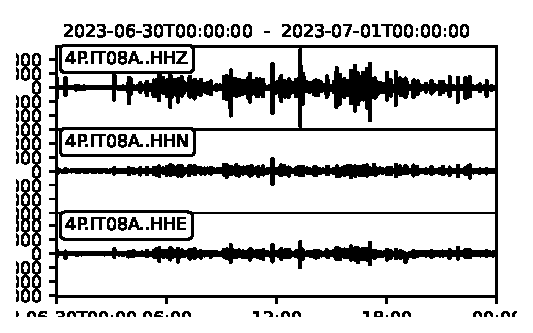
\includegraphics{4P.IT08A..230630.eps}
  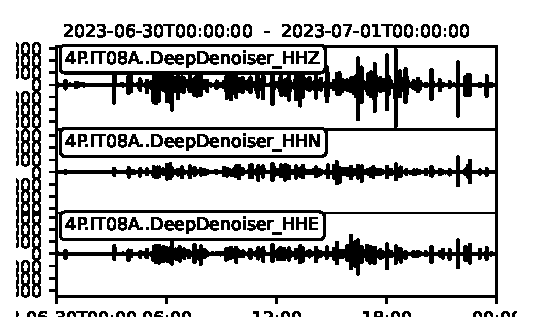
\includegraphics{D_4P.IT08A...230630.eps}
\end{figure}
\chapter{Literature Review}
ADD traditional methods for seismic wave detection and prediction
ADD a table of the hyperparameters of the different models
\input{chapters/literature_review.tex}
\chapter{Time Series Analysis}
\input{chapters/time_series_analysis.tex}
\chapter{Discussion \& Results}
\input{chapters/discussion_results.tex}
\chapter{Computation Performance}
\input{chapters/performance.tex}
\chapter{Cloud Infrastructure}
\input{chapters/cloud.tex}
\chapter{Conclusions}
\input{chapters/conclusions.tex}
\printbibliography
\end{document}